% Existing, provenance-checked outcomes only; no new experiment runs.
\section{Experiments and Discussion}\label{sec:exp}
We examine three questions: whether selecting evidence by question type
improves on transmitting the same representation for every query;
how per-sample prediction changes the accuracy--energy trade-off;
and whether a router remains useful when the receiver changes.
The evaluation separates these questions rather than assuming that
one routing policy is best in every setting.

\subsection{Experimental Setup}\label{subsec:setup}\label{subsec:tasks}
\emph{Datasets and splits.}
VisDrone-DET~\cite{zhu2021visdrone} provides $548$ aerial images,
and DroneVehicle~\cite{sun2022dronevehicle} provides $490$ images.
The questions cover presence, counting, comparison, co-presence,
and threshold. For image identifier $i$, we compute
$\mathrm{crc32}(i)\bmod100$. Values below $20$ define the test set,
values at least $80$ define validation, and the remaining values
define training. All questions and channel replays of an image
remain in one partition. VisDrone contains $343/101/104$
training/validation/test images; DroneVehicle contains $275/93/122$.
The test sets contain $936$ and $710$ questions, respectively.
Six SNR points yield $5{,}616$ decisions per VisDrone channel and
$4{,}260$ DroneVehicle decisions. Repeated log entries are deduplicated
by image, question, SNR, and branch.

The channel sweep compares fixed evidence, the type rule, and a
training-set lookup table (LUT) on VisDrone. Per-sample comparisons
use the verified AWGN records, the DroneVehicle target-data fit,
and the matched-receiver experiment below. These are distinct
evaluation settings, not interchangeable samples of one benchmark.
In particular, target-data fitting on DroneVehicle is not
VisDrone-to-DroneVehicle zero-shot transfer.

\emph{Answering and scoring.}
The YOLOv8n detector is trained on the official VisDrone training
split, disjoint from the evaluation images. It is not retrained on
DroneVehicle. The default image receiver is frozen
Qwen2-VL-2B~\cite{wang2024qwen2vl}, with greedy decoding and at most
$24$ generated tokens. The other branch applies symbolic operations
to the full received detection packet. Yes/no answers use exact
match after canonicalization. For counting, an estimate is correct
when its absolute error is at most
$\max(1,\operatorname{round}(0.1N))$, where $N$ is the true count.

Count calibration is fitted only on training images, by class and
SNR. The ratio of summed true to received training counts is clipped
to $[0.5,4]$ and retained only if it does not reduce training counting accuracy; counts below
three are left unchanged. The fitted ratios are frozen for validation
and test. An uncalibrated control is retained in the supplementary
materials. Calibration changes the receiver's counting answer, not
the sender's detector features. Learned inputs use pre-transmission
counts checked against the original detection records.

\emph{Channels and energy.}\label{subsec:energy-exp}
VisDrone uses AWGN, Rayleigh, and Rician channels at
$\{-5,0,5,10,15,20\}$\,dB; DroneVehicle uses Rician at the same SNRs.
The Rician factor is $K=6$\,dB. Bandwidth, reference window, and
radiated power are $1$\,MHz, $0.3$\,s, and $0.5$\,W.
The JPEG codec reduces quality, then resolution if necessary.
For cost reconstruction, the original codec and random seeds are
replayed on the source images. The resulting receiver JPEGs must
match the stored images byte for byte before their answers are
paired with recovered transmitted-payload costs.
All $9{,}864$ VisDrone image/SNR records and $2{,}940$
DroneVehicle image/SNR records pass this check. DroneVehicle also
passes checks on all $7{,}320$ recorded receiver-file paths.
Outages incur the full $0.3$\,s window. Detection-packet costs retain
the compact-airtime model in Section~\ref{subsec:phy}.

Table~\ref{tab:power} reports the GPU measurements underlying the
energy model. Edge VLM energy is the over-idle value of $32.31$\,J
per answer on an RTX~4060 proxy, measured on the $5$\,dB workload.
It is held fixed across the evaluated channel conditions and both
datasets, not measured anew on DroneVehicle. Sampling is approximately
$8$\,Hz over steady-state windows after a $20$\,s warm-up.
Onboard detector energy is modeled as $0.4275$\,J using a
Jetson-class power/latency envelope~\cite{nvidia2024orinnano};
it is not an embedded-device measurement. The reference amplifier
efficiency is $\eta=1$.

\begin{table}[t]\centering
\caption{GPU measurements. The detector desktop cross-check is not
the modeled onboard cost. VLM incremental energy is the reference
edge cost used in the analysis.}\label{tab:power}
\footnotesize
\begin{tabular}{@{}lrrrr@{}}\toprule
Phase & Power (W) & Time/item (s) & Incremental (J) & Total (J)\\
\midrule
Idle & 52.3 & --- & --- & ---\\
YOLOv8n cross-check & 58.7 & 0.0104 & 0.066 & 0.61\\
Qwen2-VL-2B & 107.9 & 0.581 & 32.31 & 62.72\\
\bottomrule\end{tabular}
\end{table}

Learned selectors pay detector energy for every query; the type
rule and LUT pay it only when selecting detection evidence.
Selected-sample airtime is used rather than a branch-wide mean
payload. Source encoding, router execution, symbolic decoding,
flight, sensing, queueing, and radio circuitry are excluded.
Savings therefore refer to the stated combined UAV-and-edge
account, not to measured UAV endurance.

\emph{Baselines and repeated runs.}\label{subsec:lcb}\label{subsec:stats}
The fixed-image and fixed-detection policies establish the two
answering paths. The type rule is training-free. The LUT chooses
a branch for each question-type/SNR cell using training accuracy,
with ties resolved toward detection. For paired branches with equal
sample counts this ranking is also the ranking of their Wilson
lower bounds~\cite{wilson1927probable}.
Linear routing uses two logistic correctness predictors with the
same inputs as the MLP. Its optimizer uses $400$ fixed steps,
step size $0.5$, and L2 coefficient $0.001$.
MLP hidden layers have $32$ and $16$ units; Adam uses learning rate
$0.001$, batch size $200$, and L2 coefficient $0.0001$.
Training stops after $10$ epochs without validation BCE improvement
of $10^{-4}$, with a $300$-epoch maximum, and restores the best
validation model. All MLP comparisons retain seeds $0$--$9$.

MLP results are means over these ten seeds; reported standard
deviations describe training-seed variation, not uncertainty across
independent datasets. SNR replays and questions sharing an image
are not independent observations. The comparisons below are
descriptive; small mean differences are not called statistically
significant. The supplementary materials give the provenance
boundary and additional verified controls.

\subsection{Question-Type Routing and Evidence Complementarity}
\label{subsec:main}\label{subsec:comp}\label{subsec:mechanism}
Figure~\ref{fig:f1} compares fixed evidence and type-based selection
over the VisDrone channel grid. The type rule reaches
$67.47\%$, $66.92\%$, and $67.27\%$ accuracy on AWGN, Rayleigh,
and Rician, respectively, after pooling the six SNRs.
The corresponding image accuracies are $60.43\%$, $60.15\%$,
and $60.63\%$. Thus, a simple change in answering path improves
accuracy without requiring a learned per-sample selector.

\begin{figure}[t]\centering
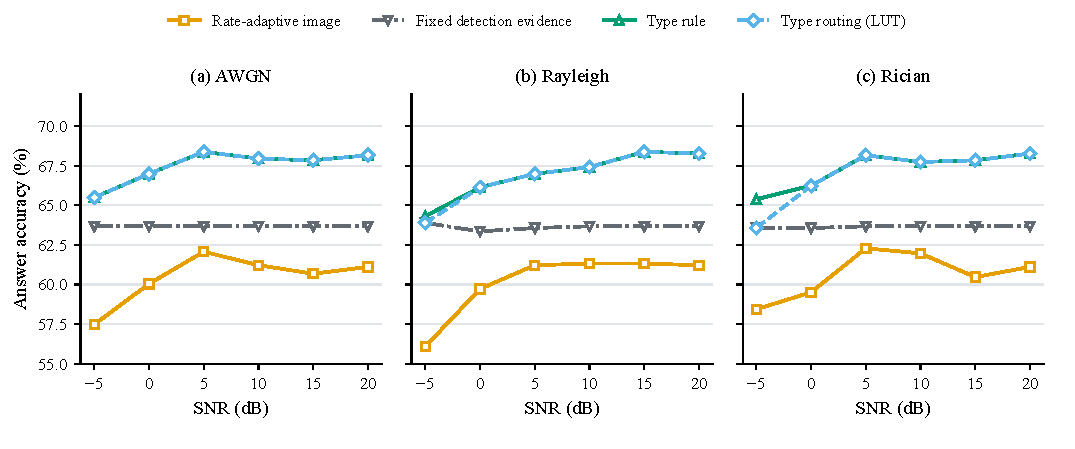
\includegraphics[width=\linewidth]{figures/evidence_final/type_routing.pdf}
\caption{VisDrone answer accuracy: $936$ questions per SNR,
with all five question types. These fixed-policy curves do not
have training-seed error bars. The LUT is fitted on training images
and is distinct from the fixed type rule.}\label{fig:f1}
\end{figure}

\begin{table}[t]\centering
\caption{VisDrone accuracy (\%) pooled over six SNRs.
Each channel contains $5{,}616$ decisions.}\label{tab:persample}
\footnotesize
\begin{tabular}{@{}lrrr@{}}\toprule
Policy & AWGN & Rayleigh & Rician\\\midrule
Image & 60.43 & 60.15 & 60.63\\
Detection evidence & 63.68 & 63.64 & 63.64\\
Type rule & 67.47 & 66.92 & 67.27\\
Training LUT & 67.47 & 66.84 & 66.97\\
\bottomrule\end{tabular}
\end{table}

The type rule uses approximately $14.46$\,J per query, compared
with $32.45$\,J for the image branch: a system saving of about
$55.4\%$. It routes $43.8\%$ of queries to the image receiver.
The LUT produces similar pooled accuracy, but chooses images less
often on the fading channels. Similar accuracy alone is therefore
not evidence that two policies have the same energy cost, nor does
it establish statistical equivalence.

Figure~\ref{fig:comp} explains why evidence selection can help.
On Rician VisDrone, detection evidence exceeds the image branch
by $18.07$, $13.62$, and $10.42$ percentage points for counting,
comparison, and co-presence. The image branch is better on presence
by $8.29$ points. Threshold is an exception to the symbolic-type
ordering: detection is lower by $1.44$ points. On DroneVehicle,
detection is better for all four count-based types, whereas the
presence gap favoring images is only $1.39$ points.
The branch ordering thus depends on the task and dataset.
These measurements motivate the rule but do not establish the
conditions of Proposition~\ref{prop:pareto} in every setting.

\begin{figure}[t]\centering
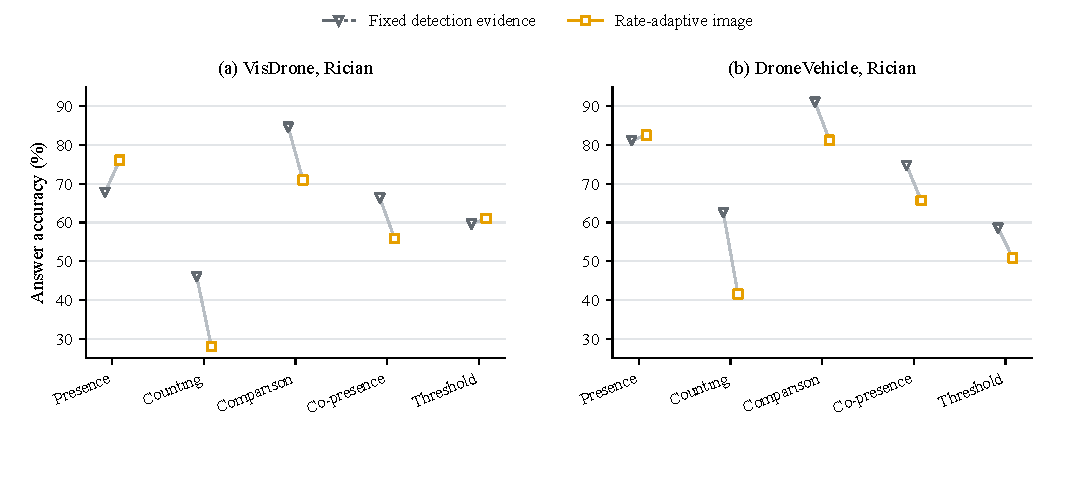
\includegraphics[width=\linewidth]{figures/evidence_final/evidence_complementarity.pdf}
\caption{Fixed-branch accuracy by question type, pooled over the
six Rician SNRs. The panels use their respective dataset questions;
they compare evidence within each dataset, not matched images
between datasets.}\label{fig:comp}
\end{figure}

\subsection{Per-Sample Routing and Energy Control}
\label{subsec:persample-exp}\label{subsec:energyctl}
A learned predictor can exploit sample differences within a question
type, but its value should be assessed against simple alternatives.
On the verified VisDrone AWGN evaluation, the unpriced MLP attains
$67.92\%\pm0.19\%$ accuracy at $13.38$\,J per query. Linear routing
attains $68.02\%$ at $11.86$\,J, while the type rule attains
$67.47\%$ at $14.46$\,J. The MLP therefore does not improve on
the linear reference in both metrics. The AWGN input ablation in
the supplementary materials also shows only small unpriced
accuracy changes. More inputs and a nonlinear predictor are not
by themselves evidence of a better system operating point.

DroneVehicle provides a separate evaluation of target-data fitting.
Table~\ref{tab:dv} retains all simple baselines. Its default MLP
improves on the type rule by $2.97$ percentage points, but consumes
$12.60$\,J instead of $11.21$\,J. In contrast, fixed detection
uses only $0.434$\,J at $72.46\%$ accuracy; the LUT selects this
branch throughout the test set. Linear routing lies close to that
low-cost endpoint. There is no single preferred policy without
an accuracy requirement or a valuation of energy.

\begin{table}[t]\centering
\caption{DroneVehicle target-data fitting on $122$ test images and
$4{,}260$ question/SNR decisions. MLP entries are ten-seed
means $\pm$ sample standard deviations.}\label{tab:dv}
\footnotesize
\begin{tabular}{@{}lrr@{}}\toprule
Policy & Accuracy (\%) & Energy (J/query)\\\midrule
Image & 64.08 & 32.442\\
Detection evidence & 72.46 & 0.434\\
Type rule & 72.93 & 11.209\\
Training LUT & 72.46 & 0.434\\
Linear, $\lambda=0$ & 72.70 & 2.810\\
Linear, validation-selected & 72.46 & 0.434\\
MLP, $\lambda=0$ & $75.91\pm0.21$ & $12.599\pm1.540$\\
MLP, validation-selected & $74.60\pm0.45$ & $4.473\pm1.406$\\
\bottomrule\end{tabular}
\end{table}

For energy control, the fixed candidate set contains zero and
$25$ logarithmically spaced prices from $10^{-5}$ to $10^{-1}$
J$^{-1}$. Each seed's operating point minimizes validation energy
among candidates whose validation accuracy is no more than one
percentage point below its own zero-price accuracy. Ties select
the smaller price. Linear routing uses the same selection procedure.
This is a relative validation constraint for each predictor, not a
common absolute accuracy target. Test labels do not select prices.

Figure~\ref{fig:f5} shows the complete DroneVehicle scan and the
validation-selected MLP point. At this point, mean accuracy is
$74.60\%$ at $4.47$\,J: $1.67$ points above the type rule and
about $60.1\%$ less accounted energy. Relative to fixed images,
the mean system saving is $86.2\%$. This result supports adjusting
the evidence choice to computation cost. It does not imply that
the MLP dominates fixed detection, which remains cheaper, or that
the selected point is globally optimal. The mean test accuracy
loss relative to the default MLP is $1.31$ points, exceeding the
one-point validation allowance. The validation criterion is not a
test-set guarantee.

\begin{figure}[t]\centering
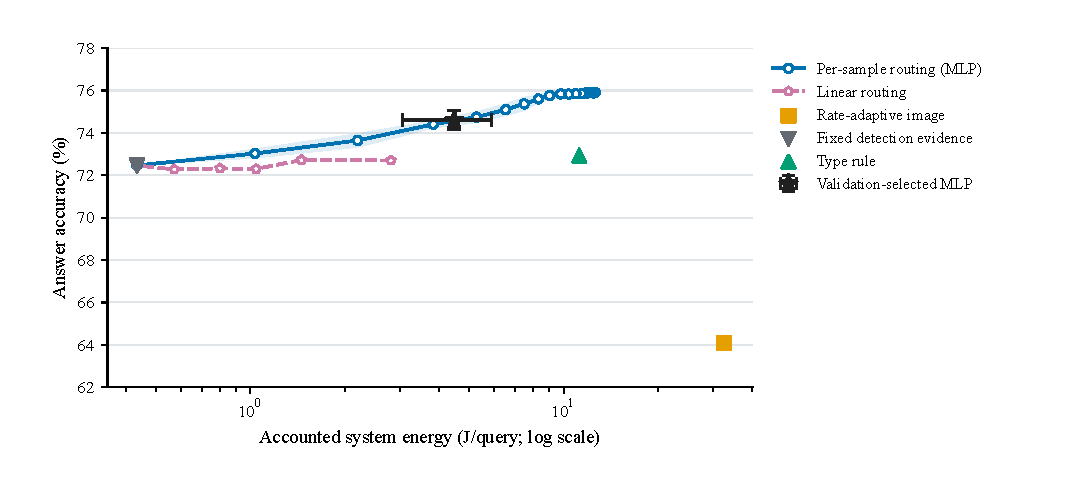
\includegraphics[width=\linewidth]{figures/evidence_final/dv_tradeoff.pdf}
\caption{DroneVehicle accuracy--energy trade-off over all $26$
fixed prices. The MLP curve gives ten-seed means at each price,
with shading for one sample standard deviation in accuracy.
The star averages seed-specific validation-selected points; its
error bars show one sample standard deviation in each coordinate.
It need not lie on the mean fixed-price curve. Energy is on a
logarithmic axis.}\label{fig:f5}
\end{figure}

\emph{System energy versus UAV energy.}\label{subsec:boundary}
Figure~\ref{fig:estack} separates the two platforms. Avoiding edge
VLM calls explains most of the reduction in total energy.
The priced MLP uses approximately $4.47$\,J in total, of which
$0.45$\,J is assigned to the UAV and $4.02$\,J to edge inference.
For fixed-image transmission, the UAV account is only $0.13$\,J
and the edge account is $32.31$\,J. The type rule's UAV cost is
$0.33$\,J. Thus, in this reference configuration, both routing
policies reduce system energy but increase modeled UAV energy
relative to fixed images. The claimed benefit is joint communication
and inference efficiency, not a demonstrated increase in flight time.

\begin{figure}[t]\centering
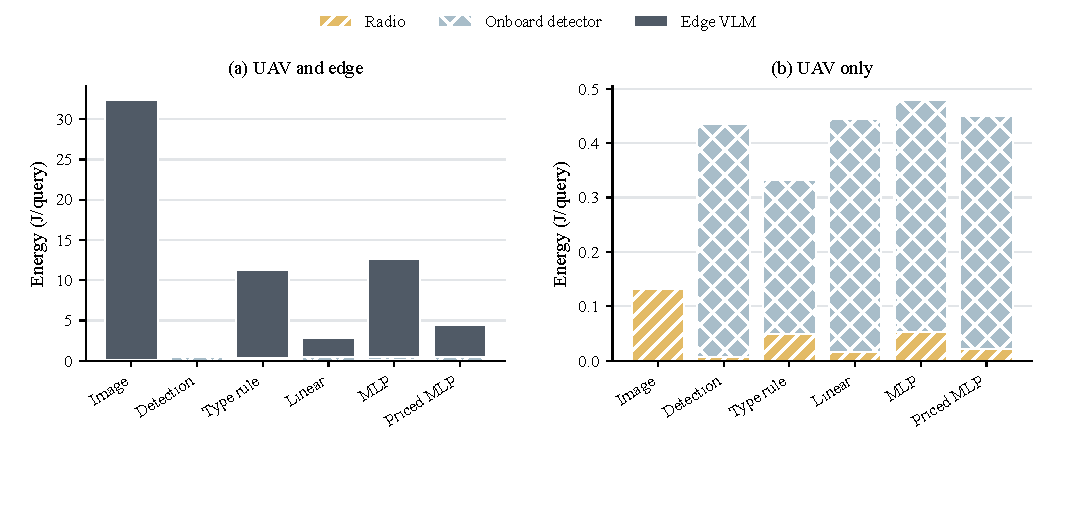
\includegraphics[width=\linewidth]{figures/evidence_final/dv_energy_components.pdf}
\caption{DroneVehicle energy components at the reported operating
points. The right panel excludes edge inference. MLP columns use
mean components over ten seeds. Detector and radio energy are
modeled; edge energy uses the fixed measured proxy. Excluded
components are stated in the experimental setup.}\label{fig:estack}
\end{figure}

\subsection{Receiver Adaptation}\label{subsec:crossvlm}\label{subsec:routerrobust}
We compare Qwen2-VL-2B, Qwen2.5-VL-3B, and SmolVLM using identical
paired question/SNR keys and byte-identical received images.
The shared detector records and training-only count calibration
are the same for all three receivers. The common partitions contain
$9{,}150/2{,}646/2{,}808$ training/validation/test decisions.
Each receiver has a separately fitted linear router and ten MLP
seeds with the same training settings. We also freeze the MLP
trained for Qwen2-VL on this common training set and apply its
unchanged decisions to the other receivers.

\begin{table}[t]\centering
\caption{Matched-receiver accuracy (\%), $\lambda=0$.
MLP entries are ten-seed means $\pm$ sample standard deviations.
Frozen-source routing uses the Qwen2-VL router without target-receiver
fitting.}\label{tab:crossvlm}
\footnotesize
\begin{tabular}{@{}lrrr@{}}\toprule
Policy & Qwen2-VL & Qwen2.5-VL & SmolVLM\\\midrule
Image & 62.93 & 62.57 & 59.29\\
Detection evidence & 67.09 & 67.09 & 67.09\\
Type rule & 69.34 & 67.31 & 67.38\\
Linear, receiver-specific & 69.59 & 68.38 & 68.13\\
MLP, receiver-specific & $69.63\pm0.38$ & $68.62\pm0.28$ & $69.29\pm0.57$\\
MLP, frozen source & --- & $68.28\pm0.43$ & $67.09\pm0.90$\\
\bottomrule\end{tabular}
\end{table}

Table~\ref{tab:crossvlm} shows that the MLP-minus-linear mean
accuracy differences are $0.04$, $0.25$, and $1.16$ points,
respectively. Receiver-specific fitting is therefore more useful
for some receivers than others. Freezing the Qwen2 router reduces
SmolVLM accuracy by $2.20$ points relative to its own MLP fit.
This supports adaptation to the answering mechanism, not arbitrary
receiver-independent routing.

The common test set includes $104$ images, but presence and counting
cover only $26$ of them. The other three types cover all $104$.
Consequently, these pooled accuracies cannot be compared directly
with the full VisDrone workload. The complete-five-type image
subset is reported separately in the supplementary materials.
No alternative-receiver energy measurements are available, so this
comparison reports accuracy and branch use, not energy savings.

\subsection{Discussion and Limitations}\label{sec:limits}
The results support question-conditioned evidence selection as a
joint choice of communication content and answering computation.
A fixed rule already captures useful differences between question
types. Per-sample prediction offers additional operating points,
but its benefit depends on the dataset, receiver, and cost assigned
to image inference. Small gains over a linear reference do not
justify a general claim for nonlinear routing.

The evaluation is limited to generated structured questions over
a modest aerial-image pool. Questions and SNR replays share images,
and image-disjoint splits do not establish independence between
nearby scenes. DroneVehicle uses only Rician and its router is
fitted on target training data. The matched-receiver workload has
unequal coverage across question types. These experiments do not
establish unrestricted-language performance or zero-shot transfer
to another aerial dataset.

Energy combines an edge-device measurement with modeled onboard
and radio costs. It assumes unbatched, per-question processing and
does not amortize detection across questions sharing an image.
The compact detection airtime and reference-window outage model
are not a validated finite-length wireless link. Source encoding,
radio circuitry, and several computation costs remain outside the
account. These assumptions limit deployment claims even when an
offline policy has lower modeled system energy. Embedded-device
measurements and online evaluation are needed to assess practical
latency and UAV battery effects.
